\documentclass{article}


% if you need to pass options to natbib, use, e.g.:
%     \PassOptionsToPackage{numbers, compress}{natbib}
% before loading neurips_2022


% % ready for submission
% \usepackage{neurips_2022}


% to compile a preprint version, e.g., for submission to arXiv, add add the
% [preprint] option:
    \usepackage[preprint]{neurips_2022}


% % to compile a camera-ready version, add the [final] option, e.g.:
    % \usepackage[final]{neurips_2022}


% to avoid loading the natbib package, add option nonatbib:
%    \usepackage[nonatbib]{neurips_2022}


\usepackage[utf8]{inputenc} % allow utf-8 input
\usepackage[T1]{fontenc}    % use 8-bit T1 fonts
\usepackage{hyperref}       % hyperlinks
\usepackage{url}            % simple URL typesetting
\usepackage{booktabs}       % professional-quality tables
\usepackage{amsfonts}       % blackboard math symbols
\usepackage{nicefrac}       % compact symbols for 1/2, etc.
\usepackage{microtype}      % microtypography
\usepackage{xcolor} % colors
\usepackage{bbm}


\title{Self-Supervised Learning with SimCLR and RotNet}

% The \author macro works with any number of authors. There are two commands
% used to separate the names and addresses of multiple authors: \And and \AND.
%
% Using \And between authors leaves it to LaTeX to determine where to break the
% lines. Using \AND forces a line break at that point. So, if LaTeX puts 3 of 4
% authors names on the first line, and the last on the second line, try using
% \AND instead of \And before the third author name.


\author{%
  Dai, Anna \\
  Duke University \\
  \texttt{anna.dai@duke.edu} \\
  \And
  Harutyunyan, Tigran \\
  Duke University \\
  \texttt{tigran.harutyunyan@duke.edu} \\
  \And
  Saikia, Deekshita \\
  Duke University \\
  \texttt{deekshita.saikia@duke.edu} \\
  % \texttt{email} \\
  % \And
  % Coauthor \\
  % Affiliation \\
  % Address \\
  % \texttt{email} \\
}


\begin{document}

\maketitle

\begin{abstract}

A major bottleneck in various use cases of deep convolutional neural networks (ConvNets) in recent days is the lack of fully labeled data. The paper aims to compare performance and learned representations of two self-supervised frameworks: SimCLR and RotNet on partially labeled data. SimCLR is a framework for contrastive Learning of image representations proposed by  Chen, et al. \cite{SimCLR}. RotNet is an unsupervised semantic feature learning framework proposed by Gidaris, et al. \cite{RotNet} to learn representations from rotated data.
We implement both frameworks with a ResNet-20 ConvNet Encoder to evaluate performance on the CIFAR-10 dataset. We find that SimCLR outperforms RotNet using linear evaluations, but RotNet in its semi-supervised state outperforms SimCLR linear evaluations. We further observe in the feature maps of the encoders from both frameworks that the RotNet encoder learns the edges of images in the first two blocks of convolutional layers, whereas the SimCLR encoders learns more comprehensive information about the images.

\end{abstract}



\section{Introduction}
\label{intro}

Convolutional neural networks (ConvNets) have unparalleled capacity to learn high level semantic image features, but usually require large amounts to labeled data to train. Labeling data comes at a high cost and is not easily scalable. The field of self-supervised learning explores how supervisory signals can be learned from the data itself, often leveraging its underlying structure, thereby reducing the need for labels for predictive tasks like classification. In recent years, approaches like contrastive learning approach with SimCLR \cite{SimCLR} and unsupervised learning with RotNet to predict image rotations \cite{RotNet} have been gaining traction. In this project, we seek to replicate these approaches with a lighter network, and benchmark their performance against an established "supervised baseline".

    % Discriminative approaches learn representations using objective functions similar to those used for supervised learning, but train networks to perform pretext tasks where both the inputs and labels are derived from an unlabeled dataset. Many such approaches have relied on heuristics to design pretext tasks (Doersch et al., 2015\cite{convnet1}; Zhang et al., 2016\cite{convnet3}; Noroozi \& Favaro, 2016\cite{convnet2}; Gidaris et al., 2018\cite{RotNet}), which could limit the generality of the learned representations. Discriminative approaches based on contrastive learning in the latent space have recently shown great promise, achieving state-of-theart results (Hadsell et al., 2006\cite{convnet4}; Dosovitskiy et al., 2014\cite{convnet5}; Oord et al., 2018\cite{convnet6}; Bachman et al., 2019\cite{convnet7}).

% \section{Related works}
% \label{related}

% WE WON'T USE THIS SECTION


\section{Methodology}


\label{method}

\subsection{Overview}
We implement both SimCLR and RotNet frameworks using a ResNet-20 backbone encoder applied on the CIFAR-10 dataset to increase comparability between the two frameworks. Our ResNet-20 encoder has three residual blocks of three convolutional layers each. We also use the vanilla ResNet-20 model as a supervised baseline model to benchmark performance. However, due to the different nature of the frameworks, we proceed to lightly tune hyper-parameters of our model, including \texttt{batch\_size}, \texttt{lr\_decay}, \texttt{optimizer}, \texttt{num\_epochs}, separately in order to achieve the best performance we can given our computational limitations. 

\subsection{SimCLR}

\subsubsection{The Contrastive Learning framework}
Contrastive learning has been shown to be a powerful approach for learning visual representations from large amounts of unlabeled data. The core idea behind contrastive learning is to use pairs of similar and dissimilar images to learn a representation that captures the differences between the images in the pair.

This framework has the following major components:

\begin{enumerate}
    \item A stochastic data augmentation module that transforms any input image into a pair of correlated views, $\mathbf{x_i}$ and $\mathbf{x_j}$ of the same input, which we call a positive pair. We sequentially apply a random resized crop, followed by a random color distortion. 
    \item The ResNet-20 base encoder network $F(\cdot)$, which extracts features from the input images and encodes them into a lower-dimensional latent space.
    \item A 2-layer MLP projection head $G(\cdot)$, which maps the latent representations to a higher-dimensional space.
    \item A contrastive loss function, which is defined for a positive pair in the following manner:
    $$ l_{i,j} = - log \frac{exp(sim(\mathbf{z_i},\mathbf{z_j})/\tau}{\sum_{k=1}^{2N} \mathbbm{1}_{[k \neq i]} exp(sim(\mathbf{z_i},\mathbf{z_j})/\tau)}$$
    where $sim(\mathbf{u},\mathbf{v}) = \mathbf{u}^\top \mathbf{v}/||u|| ||v||$ and $\tau$ denotes a temperature parameter. The indicator function $\mathbbm{1}_{[k \neq i]}$ evaluates to 1 iff $k \neq i$.
\end{enumerate}

% Insert image of SimCLR architectural diagram
\begin{figure}[!htbp]
    \centering
    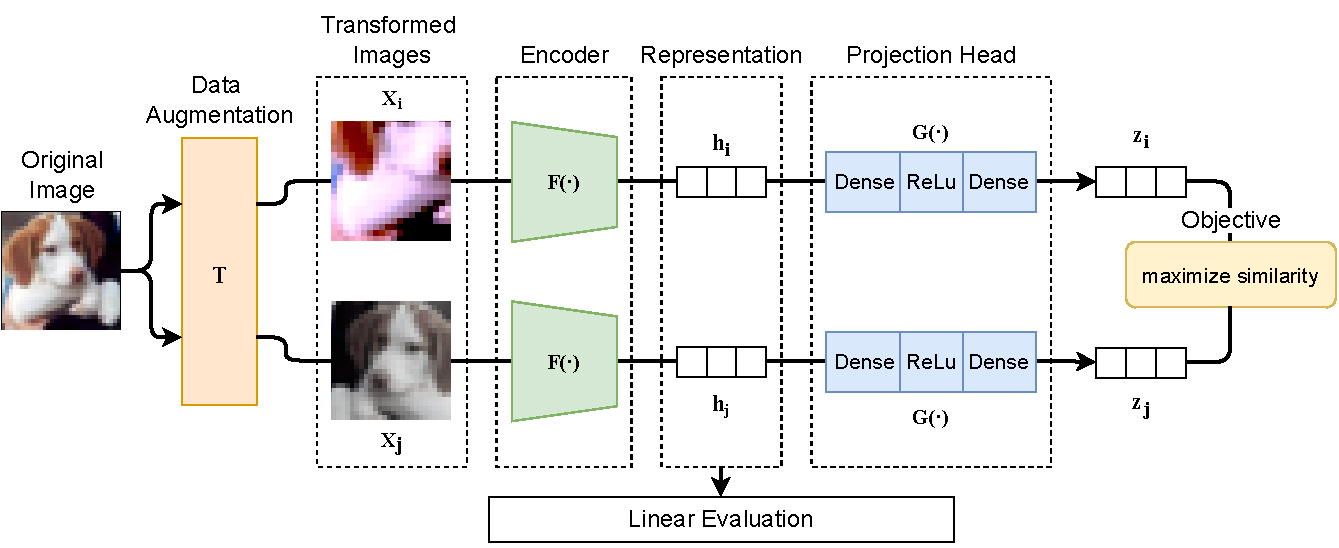
\includegraphics[width=1\linewidth]{figs/archDiag_SimCLR.png}
    \caption{Architectural diagram of SimCLR framework}
    \label{fig:archDiag_SimCLR}
\end{figure}

\paragraph{Hyper-parameters} For our implementation, we used the following settings: \texttt{EPOCHS=100}, \texttt{BATCH\_SIZE=1024}.

We optimized a temperature-scaled cross entropy-loss using a LARS optimizer with a learning rate of 0.012 and a weight decay of $1\mathrm{e}{-6}$. Further, we use a linear warm-up for the first 20 epochs, and decay the learning rate with the cosine decay schedule.

\subsection{RotNet}

The RotNet framework from paper \cite{RotNet} involves two primary steps to perform classification tasks: 1) unsupervised training on rotated images to predict its rotation and 2) semi-supervised fine-tuning process on the pre-trained unsupervised model using labeled data to classify images.

\subsubsection{Unsupervised model}

We rotate each input image (by $0^0$,$90^0$,$180^0$,$270^0$), assign labels according to its rotated angel, and train a ConvNet to learn representations of transformed input images. To effectively predict image rotations, the ConvNet must first learn to identify and locate important objects (i.e. dog's ears) in images to understand their context. It must also understand how different types of objects are typically depicted in the input images and use this information to relate the position of the objects to the dominant orientation of the image.

% Insert image of RotNet architectural diagram
\begin{figure}[!htbp]
    \centering
    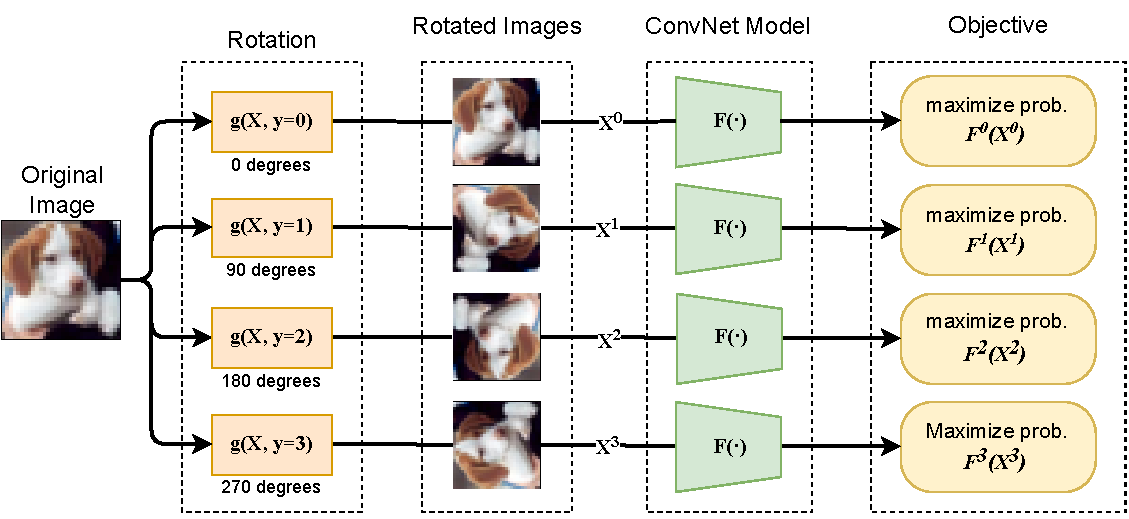
\includegraphics[width=.80\linewidth]{figs/archDiag_RotNet.png}
    \caption{Architectural diagram of RotNet framework}
    \label{fig:archDiag_RotNet}
\end{figure}

\paragraph{Hyper-parameters} For our implemention, we used the following settings: \texttt{EPOCHS=100}, \texttt{BATCH=128}, \texttt{INITIAL\_LR=0.1}, \texttt{DECAY=0.2}, \texttt{DECAY\_EPOCHS=[30, 60, 80]}. 

\subsubsection{Semi-supervised}

The architecture of the semi-supervised model is the same as the unsupervised model, except that the fully connected layer has an output size of 10 for image classification from CIFAR10.

\subsection{Evaluation Process}

To evaluate our model performance we applied linear evaluation protocol on both SimCLR and RotNet encoders. Linear evaluation one of the intended methods to evaluate model performance in the SimCLR paper \cite{SimCLR}, where we load the representations learned by the encoder, freeze all weights, and train one added linear layer with labeled data (texttt{out\_features = 10}) to classify images. It is difficult to find a fair comparison for SimCLR linear evaluation in RotNet due to the different intended use of the RotNet model for downstream tasks. Therefore, we evaluate the RotNet encoder both with the same linear process as SimCLR as well as with the intended semi-supervised setting from the RotNet paper \cite{RotNet}. Semi-supervised setting involves loading the trained encoder model, freezing only the first residual block(s), and retraining the latter block(s) with a fully-connected layer (texttt{out\_features = 10}) on labeled data.

One goal of this project is to understand how the SimCLR and RotNet frameworks perform on image classification tasks when we have partially labeled data. Therefore, we train our evaluation models on only 1\% and 10\% of our labeled data (50 images and 500 images per class respectively).

For linear evaluations, we trained the fully-connected layer over 90 epochs as instructed in the paper \cite{SimCLR} on 1\% and 10\% labels. For the RotNet semi-supervised setting, we froze the first two residual blocks of encoder and retrained the last over 80-100 epochs.



% #######
% Our goal is to train an unsupervised network using the RotNet method, and then first evaluate its performance on a classification problem with fine tuning of a fully connected layer and comparing these results with the performance of SimCLR, and then perform self-supervised training using this network with fine-tuning of the residual blocks.
% #######



\section{Experimental results}
\label{exper}

\subsection{Model accuracy}

We observe from table \ref{tbl:results} that performance improved significantly as we increase the percentage of labeled data for all models. Of the four models, the supervised baseline model observed the largest boost in model performance of 30\% from when we increased from 1\% to 10\% labels. Whereas, our SimCLR framework observed the smallest increase in prediction accuracy of around 5\%. Further, we observe that SimCLR with linear evaluations outperforms the baseline model by 15\% on 1\% labeled data, but the baseline model performs better on 10\% labeled data. 
In other words, SimCLR achieves a much better performance on almost no labels to train on but benefits less from more data labels in our implementation.

In comparison to all other models, RotNet performs the worst when linearly evaluated. It achieves a lower test accuracy than our baseline model at 1\% and SimCLR model at 10\%. This was expected as the RotNet ConvNet representations were not intended, according to the paper \cite{RotNet}, to be used in a linear manner downstream. Instead, the framework expects continued training with limited labeled data to be evaluated in its semi-supervised state. In our implementation, our semi-supervised RotNet model achieved the best model accuracy of 70.71\% with only 1\% data labels and 83.64\% with 10\%.


% Insert table of evaluation results
\begin{table}[!htbp]
    \centering
    \includegraphics[width=.60\linewidth]{figs/results}
    \vspace{0.2cm}
    \caption{Model performance on 1\% and 10\% labeled data}
    \label{tbl:results}
\end{table}

Overall, the results from our implementations are within reasonable range as compared to the two papers \cite{SimCLR} \cite{RotNet}. Our RotNet achieved results on par with the paper while our SimCLR implementation achieved lower accuracy than that from the paper on CIFAR-10. We believe variation in model performance could be due the different encoder model and our limited resources to fine-tune our hyper-parameters and run for longer epochs.

\subsection{Discussion}

From the linear evaluation experiments performed on both the SimCLR and the RotNet, we observe that SimCLR performs significantly better than the RotNet. A potential implication of this could be that the representations learned by the encoder of the SimCLR are readily applicable to downstream tasks like image classification. Whereas the RotNet would require additional fine-tuning of the last residual block (i.e. its semi-supervised setting) to increase model performance.

We visualize the representations learned at the end of each block of our ResNet-20 model from our supervised, SimCLR, and RotNet in Figure \ref{featmap} to gain insight on our results.

% Insert images of representations learned
\begin{figure}

\centering
\subfloat[Baseline Block 1]{\includegraphics[width=0.3\linewidth]{figs/BaseRep1.png}}\hfil
\subfloat[SimCLR Block 1]{\includegraphics[width=0.3\linewidth]{figs/SimRep1.png}}\hfil
\subfloat[RotNet Block 1]{\includegraphics[width=0.3\linewidth]{figs/RotRep1.png}}

\subfloat[Baseline Block 2]{\includegraphics[width=0.3\linewidth]{figs/BaseRep2.png}}\hfil 
\subfloat[SimCLR Block 2]{\includegraphics[width=0.3\linewidth]{figs/SimRep2.png}}\hfil
\subfloat[RotNet Block 2]{\includegraphics[width=0.3\linewidth]{figs/RotRep2.png}}

\subfloat[Baseline Block 3]{\includegraphics[width=0.3\linewidth]{figs/BaseRep3.png}}\hfil 
\subfloat[SimCLR Block 3]{\includegraphics[width=0.3\linewidth]{figs/SimRep3.png}}\hfil
\subfloat[RotNet Block 3]{\includegraphics[width=0.3\linewidth]{figs/RotRep3.png}}

\caption{Feature maps from last layer of each ResNet-20 residual block (4 filters shown)}\label{featmap}
\end{figure}


If we look at the first blocks in Figure \ref{featmap}(a), (b), and (c), we observe the baseline model appear to learn a variety of different features, whereas SimCLR and RotNet appear to learn more targeted features. Specifically, the RotNet model seem to focus on learning outlines of objects. The difference between the types of features learned by SimCLR and RotNet could explain why SimCLR performs better than RotNet as a linear classifier for this particular dataset.


\section{Conclusion}
\label{conc}

We have implemented a SimCLR and RotNet framework to compare their performance as an image classifier on limited labeled data from the CIFAR-10 dataset. SimCLR performed better than RotNet as a linear classifier, whereas RotNet in its semi-supervised setting outperformed all other models.

\paragraph{Acknowledgments} We would like to thank Prof. Yiran Chen, Qijia Huang and all the amazing TAs for their support on this project and their feedback on our poster (which can be found \href{https://github.com/dai-anna/SemiSupervisedBenchmarking/tree/main/poster}{here}).




\bibliography{citation.bib}
\bibliographystyle{plain}

\newpage

\appendix
\section{Appendix}

\paragraph{Contributions by team-members} The team-members made the following contributions to the project:

\begin{enumerate}
    \item \textbf{Anna Dai} - Creating the SimCLR framework, linear evaluation of Resnet-20 encoder for SimCLR
    \item \textbf{Tigran Harutyunyan} - Creating the RotNet framework, linear evaluation and semi-supervised training for RotNet
    \item \textbf{Deekshita Saikia} - Creating the SimCLR framework, tuning and pre-training of Resnet-20 encoder for SimCLR
\end{enumerate}

\paragraph{Code} The code for this project can be accessed in \href{https://github.com/dai-anna/SemiSupervisedBenchmarking}{this GitHub repository}.

\paragraph{Peer Review} We vote team D5 for best poster, named 'Contrastive Representation Learning using SimCLR and RotNet frameworks'. The poster presents results on the performances of these approaches under different self-supervised settings. The poster is well organized with plots to support their hypothesis. A variety of experiments were run and are well-balanced with their conclusions.



\end{document}